\section{Horizontal Shifting}

Now that we are working in grayscale, it is far more straightforward to manipulate aspects of the image, such as its horizontal position. Since we are dealing with a normal matrix, transforming the positions of columns requires only that we multiply the image matrix by a transformation identity matrix.

As discussed in the lab instructions, to shift an image horizontally without losing information requires the use of a transformation matrix as shown below.

    \[
      \underbrace{
        \begin{bmatrix}
          1&0&0\\
          0&1&0\\
          0&0&1\\
        \end{bmatrix}
      }_{\text{Identity Matrix}}
      \implies
      \underbrace{
        \begin{bmatrix}
          0&1&0\\
          0&0&1\\
          1&0&0\\
        \end{bmatrix}
      }_{\text{Transformation Matrix}}
    \]

    \[
      \begin{bmatrix}
        0&0&1\\
        1&0&0\\
        0&1&0\\
      \end{bmatrix}
      \cdot
      \begin{bmatrix}
        a&b&c\\
        d&e&f\\
        g&h&i\\
      \end{bmatrix}
      =
      \underbrace{
        \begin{bmatrix}
          c&a&b\\
          f&d&e\\
          i&g&h\\
        \end{bmatrix}
      }_{\text{The horizontally shifted matrix}}
    \]

    \begin{figure}[ht]
      \centering
      \begin{subfigure}{0.6\textwidth}
        \centering
        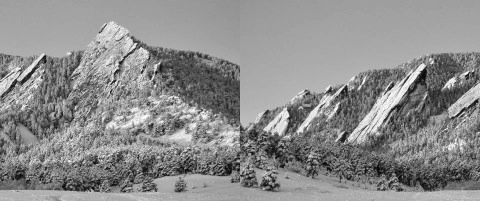
\includegraphics[scale=0.5]{./img/hsg1.png}
        \caption{Photo 1 Horizontal Shift}
        \label{fig:p1hg}
      \end{subfigure}
      \begin{subfigure}{0.3\textwidth}
        \centering
        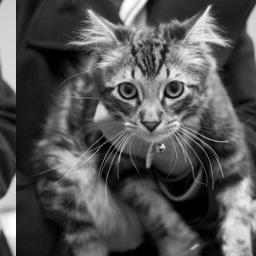
\includegraphics[scale=0.5]{./img/hsg2.png}
        \caption{Photo 2 - Horizontal Shift}
        \label{fig:p2hg}
      \end{subfigure}
      \caption{Horizontally Shifted Images}
      \label{fig:hs_images}
    \end{figure}

In the figures \eqref{fig:p1hg} and \eqref{fig:p2hg}, we have performed a shift of 240 pixels on each image. Note, for the smaller image \eqref{fig:p2hg}, the image itself is only 200 pixels wide, therefore a shift of 240 is equivalent to a shift of 40 pixels.

The python code to shift these images horizontally is below.

    \lstinputlisting[language=Python,
                    showstringspaces=false,
                    frame=single,
                    firstline=113,
                    lastline=125,
                    basicstyle=\ttfamily,
                    keywordstyle=\color{blue},
                    numbers=left,
                    commentstyle=\color{red}]{./py/analysis.py}
